\documentclass{article}
\usepackage{amsmath, amssymb,amsfonts,mdframed, tikz}
\usetikzlibrary{shapes,arrows,calc,positioning,backgrounds}
\title{Algorithms \& Complexity: Lecture 5, P vs NP \& Algorithms}
\author{Sam Barrett}

\newcommand{\T}{\texttt{T }}
\newcommand{\True}{\texttt{True }}
\newcommand{\F}{\texttt{F }}
\newcommand{\False}{\texttt{False }}
\newcommand{\NP}{\mathbf{NP}}
\renewcommand{\P}{\mathbf{P}}
\newcommand{\N}{\mathbb{N}}

\newmdtheoremenv{lemma}{Lemma}
\newmdtheoremenv{definition}{Definition}
\newmdtheoremenv{theorem}{Theorem}
\newmdtheoremenv{example}{Example}

\begin{document}
\maketitle

\section{History of Computing}
\label{sec:history}

In the 1950s to 1960s one of computer science researcher's focuses was on general ways to solve problems.

One such problem was \texttt{SAT}, is a given logical formula \(\phi\) satisfiable?

Many of the problems known at this time had polynomial running time. We know that polynomial time is ultimately always lower than exponential, for instance $1.000001^{n} > n^{10000000000}$ if $n$ is large enough. We can prove this by taking logs of both sides.

During this time polynomial time became the accepted standard of efficiency. It has many \textit{nice} properties including being \textbf{closed } under addition, multiplication and composition. I.e. if both $p$ and $q$ are polytime functions: $p(x) + q(x)$ is polytime, $p(x)\times   q(x)$ is polytime and $p(q(x))$ is polytime. We define $\P$ as the class of problems solvable in polynomial time (wrt. the size of the input).


Later, in the 1970s research moved to focus on the problems that no efficient algorithm was known to be able to solve, the set of problems that could not be included in $\P$.

Our previous example \texttt{SAT} cannot be brute forced in polynomial time. If given $N$ variables in $M$ clauses, we must make $2^{N}$ truth assignments, checking each of the $M$ clauses in $O(N)$ time resulting in overall running time in $O(2^{N}\cdot N \cdot M)$, clearly this is in $\mathbf{EXP} $.

Research started to focus on trying to prove that there is no solution in $\P$ for \texttt{SAT}.

In so doing a new class was defined, $\NP$. The class of problems where we can verify a potential solution, or certificate, in polynomial time.

\textbf{\underline{How much harder is solving compared with verifying?}}

Given that we define $\P$ as the class of problems with solutions in polytime, and $\NP$ is the class of problems for which we can verify a potential solution in polytime, clearly $\P \subseteq \NP$ as solving can be seen as a very difficult way of verifying.

But what about the opposite direction? Say we can verify potential solutions in $n^{12}$ time, how long would it take us to \textbf{solve} the problem? If we can solve this in some polynomial amount of time $n^{k}$ then we have shown that $\P = \NP$!


\section{From \texttt{SAT} to graphs}

\begin{definition}(Independent Set)
  Given an undirected graph $G = (V,E)$ on $n$ vertices, find a set $X$ of maximal size such that no pair of vertices in $X$ form an edge
\end{definition}

We can reduce the independent set problem to \texttt{SAT}:

\begin{itemize}
  \item Take an instance $I$  of 3-\texttt{SAT} with $N$ variables and $M$ clauses
  \item Build a graph $G$ on 3$M$ vertices as follows:
        \begin{itemize}
          \item Introduce triangle for each clause
          \item Add conflicts to ensure every variable is not both \True and \False
        \end{itemize}
        \item \underline{Claim:} $I$ is satisfiable iff $G$ has an independent set of size $M$
\end{itemize}

This reduction is in polytime meaning that the Independent set problem is also in $\NP$

\subsection{Example}

Suppose we have an $I = \underbrace{(x_{1} \vee x_{2}\vee \bar{x_{3}})}_{c_{1}} \wedge \underbrace{(x_{2} \vee \bar{x_{4}} \vee \bar{x_{1}})}_{c_{2}} \wedge \underbrace{(x_{3} \vee x_{1} \vee \bar{x_{2}})}_{c_{3}}$

We can convert each clause into a separate triangle:

$c_{1}$:

\begin{center}
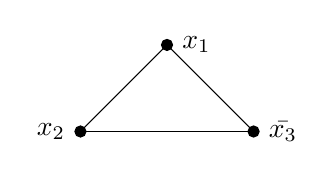
\begin{tikzpicture}
  \node[circle, draw=black, fill=black, minimum size= 4pt, inner sep=0pt, outer sep=0pt, label=right:$x_{1}$] (x1) {} ;
  \node[circle, draw=black, fill=black, minimum size= 4pt, inner sep=0pt, outer sep=0pt, below left = of x1, label=left:$x_{2}$] (x2) {};
  \node[circle, draw=black, fill=black, minimum size= 4pt, inner sep=0pt, outer sep=0pt, below right = of x1, label=right:$\bar{x_{3}}$] (x3) {};

  \draw (x1) -- (x2);
  \draw (x2) -- (x3);
  \draw (x1) -- (x3);

\end{tikzpicture}
\end{center}

$c_{2}$:


\begin{center}
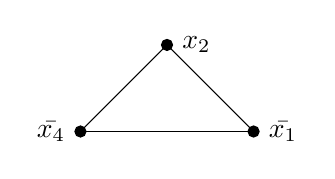
\begin{tikzpicture}
  \node[circle, draw=black, fill=black, minimum size= 4pt, inner sep=0pt, outer sep=0pt, label=right:$x_{2}$] (x2) {} ;
  \node[circle, draw=black, fill=black, minimum size= 4pt, inner sep=0pt, outer sep=0pt, below left = of x2, label=left:$\bar{x_{4}}$] (x4) {};
  \node[circle, draw=black, fill=black, minimum size= 4pt, inner sep=0pt, outer sep=0pt, below right = of x2, label=right:$\bar{x_{1}}$] (nx1) {};

  \draw (x2) -- (x4);
  \draw (x2) -- (nx1);
  \draw (x4) -- (nx1);

\end{tikzpicture}
\end{center}

$c_{3}$

\begin{center}
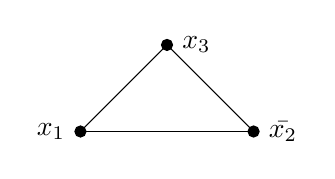
\begin{tikzpicture}
  \node[circle, draw=black, fill=black, minimum size= 4pt, inner sep=0pt, outer sep=0pt, label=right:$x_{3}$] (x3) {} ;
  \node[circle, draw=black, fill=black, minimum size= 4pt, inner sep=0pt, outer sep=0pt, below left = of x3, label=left:$x_{1}$] (x1) {};
  \node[circle, draw=black, fill=black, minimum size= 4pt, inner sep=0pt, outer sep=0pt, below right = of x3, label=right:$\bar{x_{2}}$] (nx2) {};

  \draw (x3) -- (x1);
  \draw (x1) -- (nx2);
  \draw (x3) -- (nx2);

\end{tikzpicture}
\end{center}

Now we must add our conflicts. We do this by connecting conflicting variables.

\begin{center}
  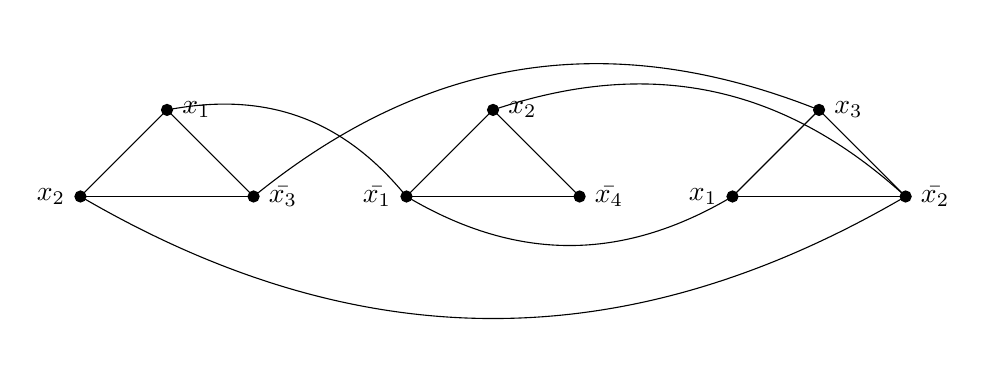
\begin{tikzpicture}

   % C1
  \node[circle, draw=black, fill=black, minimum size= 4pt, inner sep=0pt, outer sep=0pt, label=right:$x_{1}$] (x1) {} ;
  \node[circle, draw=black, fill=black, minimum size= 4pt, inner sep=0pt, outer sep=0pt, below left = of x1, label=left:$x_{2}$] (x2) {};
  \node[circle, draw=black, fill=black, minimum size= 4pt, inner sep=0pt, outer sep=0pt, below right = of x1, label=right:$\bar{x_{3}}$] (nx3) {};

  \draw (x1) -- (x2);
  \draw (x2) -- (nx3);
  \draw (x1) -- (nx3);

  %C2

  \node[circle, draw=black, fill=black, minimum size= 4pt, inner sep=0pt, outer sep=0pt, right= 4cm of x1, label=right:$x_{2}$] (c2x2) {} ;
  \node[circle, draw=black, fill=black, minimum size= 4pt, inner sep=0pt, outer sep=0pt, below left = of c2x2, label=left:$\bar{x_{1}}$] (nx1) {};
  \node[circle, draw=black, fill=black, minimum size= 4pt, inner sep=0pt, outer sep=0pt, below right = of c2x2, label=right:$\bar{x_{4}}$] (nx4) {};

  \draw (c2x2) -- (nx1);
  \draw (nx1) -- (nx4);
  \draw (c2x2) -- (nx4);

  %C3

  \node[circle, draw=black, fill=black, minimum size= 4pt, inner sep=0pt, outer sep=0pt, right= 4cm of c2x2, label=right:$x_{3}$] (c3x3) {} ;
  \node[circle, draw=black, fill=black, minimum size= 4pt, inner sep=0pt, outer sep=0pt, below left = of c3x3, label=left:$x_{1}$] (c3x1) {};
  \node[circle, draw=black, fill=black, minimum size= 4pt, inner sep=0pt, outer sep=0pt, below right = of c3x3, label=right:$\bar{x_{2}}$] (nx2) {};

  \draw (c3x3) -- (c3x1);
  \draw (c3x1) -- (nx2);
  \draw (c3x3) -- (nx2);


  \draw (x2) edge[bend right] node {} (nx2);
  \draw (c3x3) edge[bend right] node {} (nx3);
  \draw (x1) edge[bend left] node {} (nx1);
  \draw (c3x1) edge[bend left] node {} (nx1);
  \draw (c2x2) edge[bend left] node {} (nx2);


\end{tikzpicture}
\end{center}

\section{Algorithmic paradigms to cope with $\NP$-hardness}

Assuming $\P \neq \NP$, a problem $X$ being $\NP$-hard implies that we cannot have an algorithm \texttt{ALG} for it which satisfies both of the following properties:

\begin{itemize}
  \item \texttt{ALG} is always correct
  \item \texttt{ALG} runs in polytime
\end{itemize}

This has lead to the development of new \textbf{algorithmic paradigms} including:
\begin{enumerate}
  \item Exact Exponential algorithms

        Here we are focused on producing correct results, no matter the time complexity cost.

  \item Polytime approximation algorithms

        Here we want to focus on having a polynomial running time, to do this we relax our first requirement and allow our algorithm to return only approximately correct results in some cases.

  \item Parameterised algorithms

        Before trying to solve a problem optimally we can fix a parameter $k$ and using this we can now reevaluate running time with respect to both the length of the input as we always have but also our fixed parameter $k$.

  \item Polytime randomisation algorithms

        Here our algorithm must still run in polytime, and instead of always being correct we say that it must be correct with a given probability.
\end{enumerate}


\subsection{Exact exponential algorithms}
\label{subsec:exact-exponential}

This approach essentially tries to answer the question: \textit{``Can we do better than brute force, even if it still uses exponential time?''}

\subsubsection{Vertex Cover}

\begin{definition}
  Given an undirected graph $G = (V,E)$ on $n$ vertices, find a set $X$ of minimum size such that each edge of $G$ has at least one endpoint in $X$
\end{definition}

The brute force approach to this problem runs in $2^{n}\cdot n^{O(1)}$ time. Can we design an $1.99^{n} \cdot n^{O(1)}$ time algorithm?

For instance the graph:

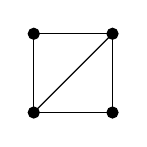
\begin{tikzpicture}
  \node[circle, draw=black, fill=black, minimum size= 4pt, inner sep=0pt, outer sep=0pt] (n1) {} ;
  \node[circle, draw=black, fill=black, minimum size= 4pt, inner sep=0pt, outer sep=0pt, right of=n1] (n2) {} ;
  \node[circle, draw=black, fill=black, minimum size= 4pt, inner sep=0pt, outer sep=0pt, below of=n2] (n3) {} ;
  \node[circle, draw=black, fill=black, minimum size= 4pt, inner sep=0pt, outer sep=0pt, below of=n1] (n4) {} ;

  \draw (n1) -- (n2);
  \draw (n2) -- (n3);
  \draw (n3) -- (n4);
  \draw (n4) -- (n1);
  \draw (n4) -- (n2);
\end{tikzpicture}

Has a solution of:

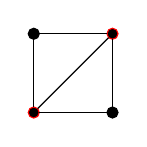
\begin{tikzpicture}
  \node[circle, draw=black, fill=black, minimum size= 4pt, inner sep=0pt, outer sep=0pt] (n1) {} ;
  \node[circle, draw=red, fill=black, minimum size= 4pt, inner sep=0pt, outer sep=0pt, right of=n1] (n2) {} ;
  \node[circle, draw=black, fill=black, minimum size= 4pt, inner sep=0pt, outer sep=0pt, below of=n2] (n3) {} ;
  \node[circle, draw=red, fill=black, minimum size= 4pt, inner sep=0pt, outer sep=0pt, below of=n1] (n4) {} ;

  \draw (n1) -- (n2);
  \draw (n2) -- (n3);
  \draw (n3) -- (n4);
  \draw (n4) -- (n1);
  \draw (n4) -- (n2);
\end{tikzpicture}

Where $X=2$.

The brute force approach to finding this would be to enumerate all subsets of vertex set of $G$, $V$ in increasing sizes and for each subset, checks in polynomial time whether it is a vertex cover. This check is performed simply by checking whether every element in $E$ is connected to at least one of the vertices in the subset.

We can make observations which can allow us to improve upon this approach. One such observation is that there is no point in adding a vertex of degree 1 to our vertex cover, it can never connect to more points than its unique neighbour (the vertex on the other end of the edge), so we add the unique neighbour instead.

So we say that we only add vertices of degree $\geq 2$ to the vertex cover. This, for every potential vertex, introduces a binary choice as to whether we add it to the vertex cover. Using this we define $T(n)$ as the time needed to solve the vertex cover on graphs with $n$ vertices. We can therefore say that $T(n) \leq T(n-1) + T(n-3)$.

We derive this inequality by saying:

\begin{itemize}
  \item $T(n-1)$ is \textit{spawned} as a sub problem when we \textit{take} $v$ into the vertex cover, we reduce the size of $V$ by 1
        \item Alternatively, if we do \textbf{not} add $v$ to the vertex cover, we \textbf{must} add all $\geq2$ neighbours to the VC, so the number of vertices to consider in the subproblem has decreased by \textbf{at least} 3.
\end{itemize}

We can solve this inequality by setting $T(n)$ equal to $x^{n}$ which gives us $x^{0} - x^{2} -1 = 0 $, solves to $1.47^{n} \cdot n^{O(1)}$.


\subsection{Polynomial time approximation algorithms}

Again looking at our Vertex Cover problem, can we find a vertex cover with has size at most 10 times that of the minimum vertex cover ? Can we do it in $n^{O(1)}$ time?

Do do this we must first find a maximal set $M$ of pairwise disjoint edges. This \textbf{can} in fact be found in polynomial time!

Using this we can output a solution $R$ which has both endpoints of each edge from $M$. By definition $R$ is a vertex cover, albeit not a minimal vertex cover. We can see that if \texttt{OPT} is a vertex cover of minimum size, then $|R|\leq 2\cdot |\texttt{OPT}| $.

We have designed a 2-approximation for the Vertex Cover problem in $n^{O(1)}$ time, nothing better is known.

\subsection{Parameterised algorithms}

To look at this approach we have to tweak the definition of our Vertex Cover problem:

\begin{definition}(Parameterised Vertex Cover)
 Given an undirected graph $G=(V,E)$ on $n$ vertices and an integer $k$, goes $G$ have a vertex cover of size $\leq k$?
\end{definition}

This can be thought of as the question: \textit{``Given a parameter $k$, how fast can we check whether there is a vertex cover of size $k$?} . Here we are not concerned with the size of the minimum vertex cover, rather we are concerned with being able to say whether the minimal vertex cover lies above or below $k$

An algorithm has been found which runs in $2^{k}\cdot n^{O(1)}$ time.

\subsection{Polynomial time randomisation algoriths}

\begin{definition}(Max Cut)
  Given an undirected graph $G=(V,E)$ on $n$ vertices, find a set $X$ which maximises the number of edges which have one endpoint in $X$ and the other endpoint in $V \backslash X$
\end{definition}


We can define a 0.5-approximation algorithm. Since the goal with this problem is to maximise, the approximation ratio is usually written as $<1$. This algorithm works by flipping a coin to decide which side of the partition each vertex goes to. We expect half of the edges to be in the \textit{cut}.

This algorithm runs in $n^{O(1)}$ time.

This approach can be de-randomised by starting with any arbitrary partition, and for each vertex if it has strictly more neighbours in the same side then move it to the other side. This re-shuffling must be finite as eventually exactly half the edges are in each cut.

The best known result for this problem is a 0.86-approximation.


\end{document}
